%!TEX root = /Users/louis/Documents/PhD/Deliverables/Thesis/thesis.tex

\section{Research Hypothesis and Method}
\label{sec:hypothesis}

The research presented in this thesis explores the hypothesis below. The emboldened terms are potentially ambiguous, and their definition follows the hypothesis.

\begin{quote}
\emph{In existing MDE projects, the evolution of \textbf{MDE development artefacts} is typically managed in an ad-hoc manner with little regard for re-use. Dedicated structures and processes for \textbf{managing evolutionary change} can be designed by analysing evolution in existing MDE projects. Furthermore, supporting those dedicated structures and processes in contemporary MDE environments is beneficial in terms of increased \textbf{productivity} for software development activities pertaining to the management of evolutionary change.}
\end{quote}

In this thesis, the terms below have the following definitions:

\paragraph{MDE development artefacts.} Compared to traditional approaches to software engineering, MDE uses additional development artefacts as first-class citizens in the development process. The additional development artefacts particular to MDE include models and modelling languages, as well as model management operations (such as model transformations). Chapter~\ref{Background} describes models, modelling languages and model management operations in more detail.

\paragraph{Managing evolutionary change.} Contemporary computer systems are constructed by combining numerous interdependent artefacts. Evolutionary changes to one artefact can affect other artefacts. For example, changing a database schema might cause data to become invalid with respect to the database integrity constraints, and changing source code may require recompilation of object code to ensure the latter is an accurate representation of the former. Managing evolutionary change typically comprises three related activities: \emph{identifying} when a change has occurred, \emph{reporting} the effects of a change, and \emph{reconciling} affected artefacts in response to a change. Chapter~\ref{LiteratureReview} reviews existing approaches to managing evolutionary change.

\paragraph{Productivity} is a measure of the output from a process, per unit of input \cite{beattie07economics}. For example, the productivity of data entry might be measured by counting the number of characters produced per typist per hour. An Optical Character Recognition (OCR) system might increase data entry productivity, but this is likely to be dependent on many factors, including: the accuracy and capabilities of the OCR system, the speed and accuracy of each typist, and the legibility and consistency of the data. Managing and measuring the productivity of software engineering is challenging. Division of labour, for example, can decrease productivity in software engineering as evidenced by Brooks's eponymous law (``adding manpower to a late software project makes it later'') \cite{brooks95mythical}. This thesis investigates the productivity of small, well-defined software development activities, and not the productivity of software engineering projects.

\subsection{Thesis Objectives}
The objectives of the thesis are to:

\begin{enumerate}
	\item Identify and analyse the evolution of MDE development artefacts in existing projects.
	\item Investigate the extent to which existing structures and processes can be used to manage the evolution of MDE development artefacts. 
	\item Propose and develop prototypes of new structures and processes for managing the evolution of MDE development artefacts, and integrate those structures and processes with a contemporary MDE development environment.
	\item Evaluate the proposed structures and processes for managing evolutionary change, particularly with respect to productivity.
\end{enumerate}

\subsection{Research Method}
\label{sec:research_method}
To explore the hypothesis outlined above, the thesis research was conducted using the method described in this section and summarised in Figure~\ref{fig:research_method}. The shaded boxes represent the three \emph{phases} of research, which are described below. The unshaded boxes represent inputs and outputs to those phases.

\begin{figure}[htbp]
  \begin{center}
    \leavevmode
    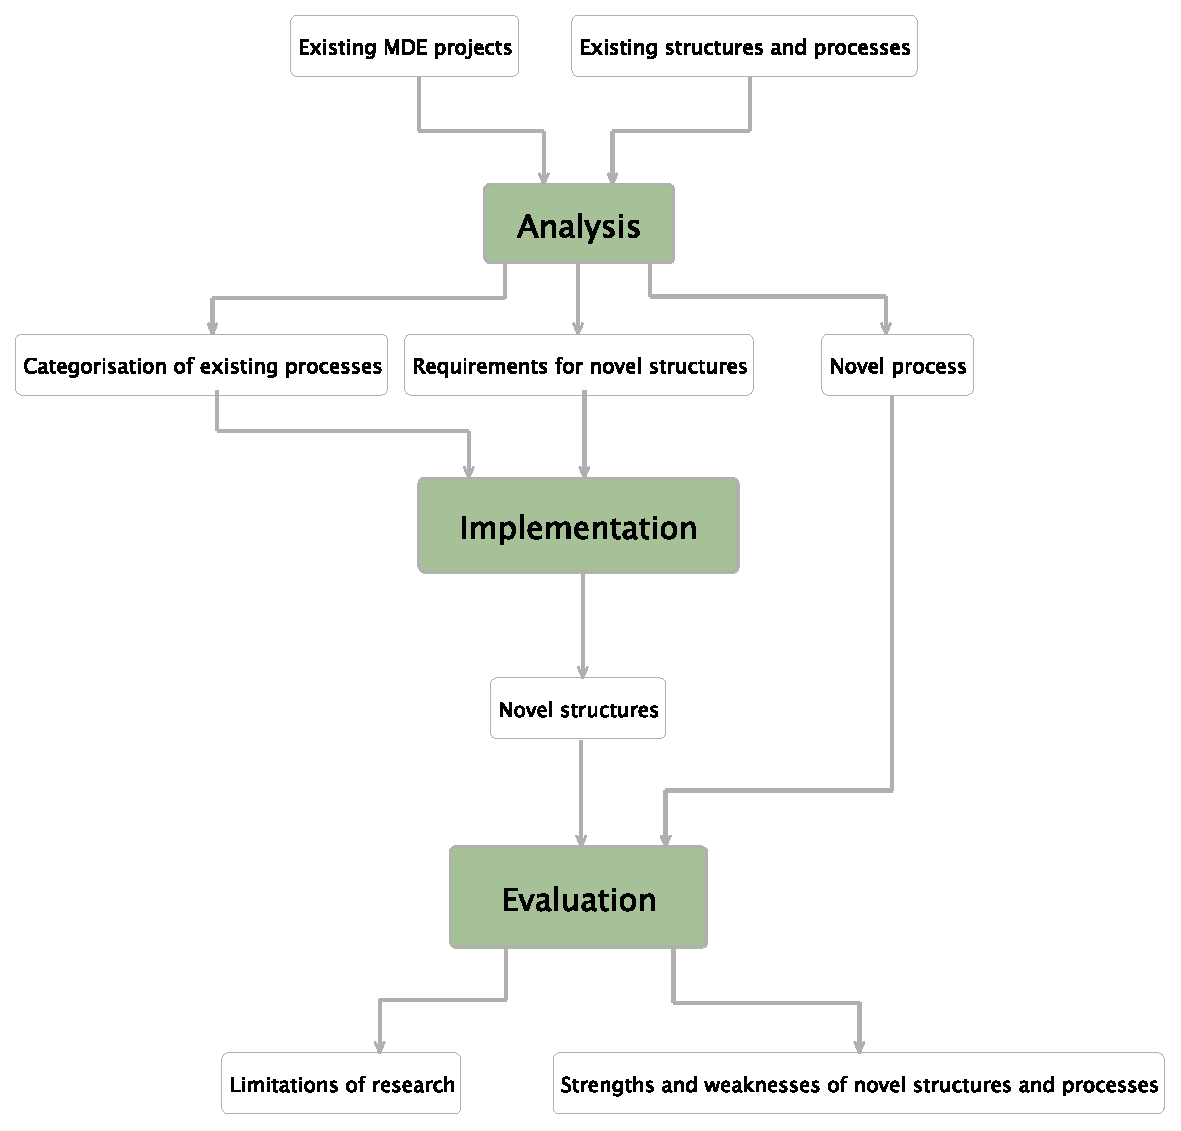
\includegraphics[width=12cm]{1.Introduction/images/method.pdf}
  \end{center}
  \caption{Overview of the research method.}
  \label{fig:research_method}
\end{figure}


Firstly, the \emph{analysis} phase involved studying the evolution of MDE development artefacts in existing projects. The results of the analysis phase were used to determine a category of evolution that lacked support in contemporary MDE development environments, \emph{model-metamodel co-evolution} or, simply \emph{co-evolution}. Co-evolution examples from existing MDE projects were used to categorise existing processes for managing co-evolution, and to formulate requirements for new structures and processes for managing co-evolution. The analysis phase also led to the identification of \emph{user-driven co-evolution}, a process for managing co-evolution that has not previously been recognised in the co-evolution literature.

The \emph{implementation} phase involved proposing, designing and implementing prototypes of novel structures for managing co-evolution, and integrating the prototypical structures with a contemporary MDE environment. The co-evolution examples identified in the analysis phase were used for testing the implementation of the structures.

The \emph{evaluation} phase involved assessing the novel structures for managing co-evolution by comparison to existing structures, and demonstrating the novel process. Evaluation was performed using further examples of co-evolution. To mitigate a possible threat to the validity of the research, the examples used in the evaluation phase were different to those used in the analysis phase. The strengths and weaknesses of the novel and existing structures and processes were synthesised from the comparisons, particularly with respect to the productivity of the development activities that are used to manage co-evolution.

A similar method was used successfully in \cite{dig07thesis} to explore the extent to which component-based applications can be automatically evolved. Initially, \cite{dig06apis} conducted \emph{analysis} to identify and categorise evolution in five existing component-based applications, with the hypothesis that many of the changes could be classified as behaviour-preserving. By using examples from the survey, \cite{dig06detection} were able to \emph{implement} an algorithm for automatically detecting behaviour-preserving changes. The algorithm was then used to implement tools for migrating code in a distributed and collaborative software development environment \cite{dig06automatic}, and for analysing the history of component-based applications \cite{dig07cms}. The latter facilitated better understanding of program evolution, and refinement of the detection algorithm. Finally, \cite{dig07thesis} \emph{evaluated} the tools and detection algorithm by application to three further component-based applications.